\documentclass[]{report}
\usepackage{graphicx}
\usepackage{blindtext}
\usepackage[inline]{enumitem}
\usepackage{xcolor}
\usepackage{listings}

% Title Page
\title{Øvelse 4 - DC-motoren som positionsservo}
\author{Jonas Lind\\Marcus Andersen\\Tais Hjortshøj}


\begin{document}
\maketitle

\chapter{}
\section{Øvelsesobjekt}
Øvelsesobjektet består af en færdigmonteret motorstand. Motor, tachometer, gear, ekstra inertibelastning og nu også potentiometeret til måling af vinkeldrejning, er monteret samlet og udgør reguleringsobjektet. 
Tillige bruges oscilloscope, funktionsgenerator, Power Amplifier og en Control box, hvor regulator-parametre kan realiseres.

\section{Formål}
\begin{itemize}
	\item at opbygge et positions reguleringssystem (positionsservo)
	\item ud fra givne dynamiske og statiske systemkrav, at dimensionere en Lead-regulator
	\item at afprøve virkningen af en P-, PI- og Lead regulator, realiseret analogt i laboratoriet
	\item simulering i Matlab
\end{itemize}

\section{Systemoversigt}
\begin{figure}[h]
	\centering
	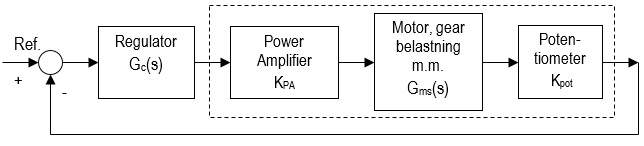
\includegraphics[width=1\linewidth]{graphics/systemoversigt}
	\caption{Systemoversigt}
	\label{fig:systemoversigt}
\end{figure}
\noindent Processen er nu forstærker og motoropstilling med potentiometer, indrammet i systemoversigten ovenfor. 
I vil i øvelse 2 have målt forskellige modelparametre, men nu tager vi et fælles udgangspunkt og antager at:\\
\newline
\begin{tabular}{llllll} 
	$R_{a}$ & $18 \,ohm$ & $K_{t} = K_{b}$ & $0,044 \,Nm/A, V/s$ & J & $3,4*10^{-6}$ \\ 
	D & $ 6*10^{-6} \,Nms$ & $K_{ms}$ &  $720 \,(Vs)-1$ & $\tau_{ms}$ & $30 \,ms$ \\ 
\end{tabular} \\ \\
\newline Medbring et USB memory stick, til at gemme scope-billeder på.

\section{Forberedelse}
Åbensløjfe overføringsfunktionen for det samlede system er:\\
\begin{figure}[h]
	\centering
	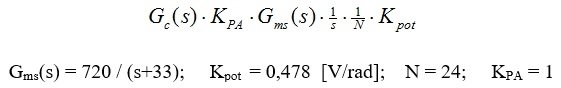
\includegraphics[width=0.8\linewidth]{graphics/openloop_tf}
	\label{fig:openlooptf}
\end{figure}

\begin{enumerate*}[label={\alph*)}]
	\item Idet Gc(s) er en konstant, KC , ønskes ved simulering fundet den største værdi, for hvilken lukketsløjfe systemet har et oversving < 5\%. Brug Matlab. Iagttag settlingtime, oversving og stationære fejl. Plot for KC-værdien amplitude- og fasekarakteristik, og find den tilhørende fasemargin, φm og fasemarginsfrekvens, ωφm . Brug Matlab-ordren margin.\\	
	\newline \item Systemet er et type 1, og vil have en stationær fejl  fra 0 for rampeinput. 
	Idet referencen er en trekantkurve, der går ±200 mV med frekvensen  0,5 Hz,  ønskes den stationære fejl, e(), beregnet med værdierne fra a)\\
	\newline Den stationære fejl kan forbedres ved øget DC-forstærkning, og vi vil forsøge med PI-regulatoren: $G_{c}(s) = \frac{(s+10)}{s}$, der repræsenterer det største TI, der kan indstilles på Control box. \\
	\item Simuler step og ramperesponset med og uden PI-regulatoren indkoblet og forklar forløbet ud fra Bodeplottet i a) og det for systemet med PI-regulatoren.\\
	\newline Efterfølgende anvendes PI-regulatoren ikke.\\
	\newline \item Idet KC forøges til ca. 90 gg findes tilhørende φm og ωφm . Indtegn situationen i et Bodeplot og kontroller med et stepresponse. Brug Matlab. Iagttag settling time og oversving.\\
	\newline \item Dimensioner en Lead-regulator så systemet har et oversving < 5\% som i a), men med samme fasemarginsfrekvens som i d). Indtegn situationen i et Bodeplot og kontroller med et stepresponse. Brug Matlab. Iagttag settling time og oversving.\\
\end{enumerate*}
\newline a) Iagttag settlingtime, oversving og stationære fejl. Kc sættes til 39, da den ved højere værdier giver mere end 5\% overshoot. 39 giver følgende graf og et overshoot på 4,69\%, en settling time på 0,253s uden stationær fejl.
\begin{figure} [h]
	\centering
	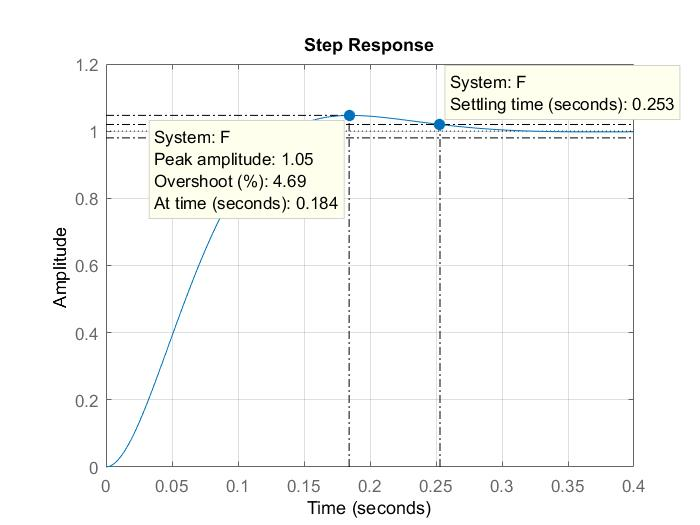
\includegraphics[width=0.68\linewidth]{graphics/a_steprespons}
	\caption{Step Response}
	\label{fig:asteprespons}
\end{figure}
\newline Amplitude- og fasekarakteristik for Kc værdien. Fasemargin på 65 grader og fasemarginsfrekvensen på 15,1 rad/s. \\
\begin{figure}[h]
	\centering
	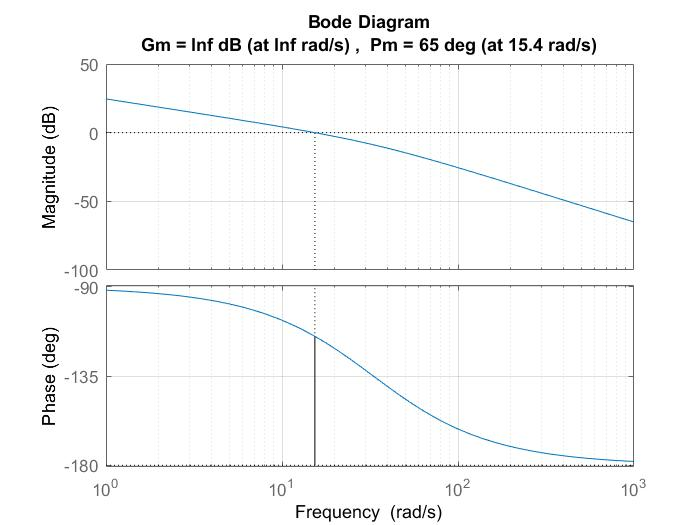
\includegraphics[width=0.68\linewidth]{graphics/a_fasekarakteristik}
	\caption{Bode Diagram}
	\label{fig:afasekarakteristik}
\end{figure}
\newpage \noindent b) Den stationære fejl findes ved først at udregne hastighedskonstanten med denne formel.\\
Fejlen er så:\\
\newline $E = \frac{Haeldning}{K_{v}}$\\
\newline c)\\
\newline d) Kc forøges til ca. 90 gg. Iagttag settling time og oversving. Det giver følgende graf og et overshoot på 19,7\%, en settling time på 0,231s uden stationær fejl.
\begin{figure}[h]
	\centering
	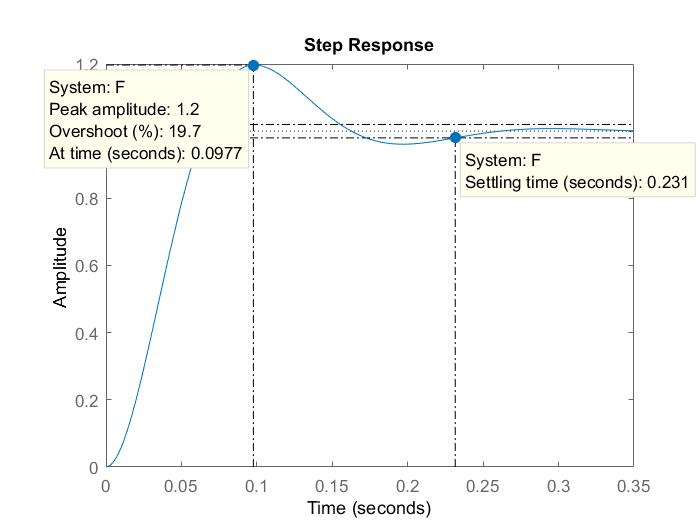
\includegraphics[width=0.68\linewidth]{graphics/d_steprespons}
	\caption{Bode Diagram}
	\label{fig:dsteprespons}
\end{figure}
\newline Amplitude- og fasekarakteristik for Kc værdien. Fasemargin på 48,4 grader og fasemarginsfrekvens på 29,1 rad/s. 
\begin{figure}[h]
	\centering
	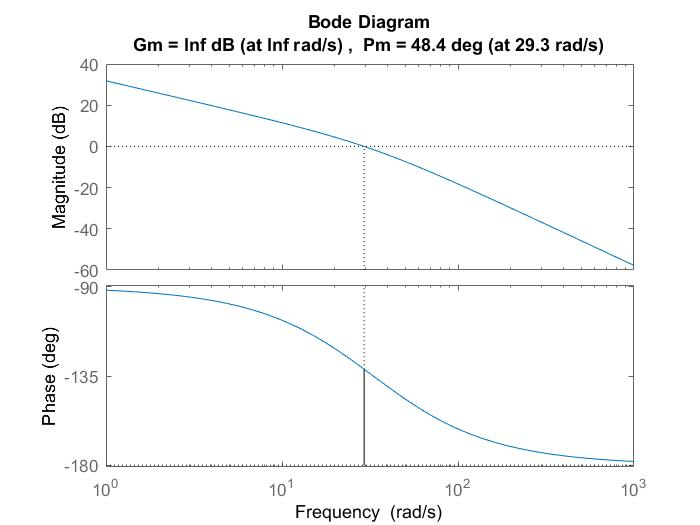
\includegraphics[width=0.68\linewidth]{graphics/d_fasekarakteristik}
	\caption{Bode Diagram}
	\label{fig:dfasekarakteristik}
\end{figure}
\newline \noindent Den Lead-regulator, der kan realiseres på Controler box’en er:
\begin{figure}[h]
	\centering
	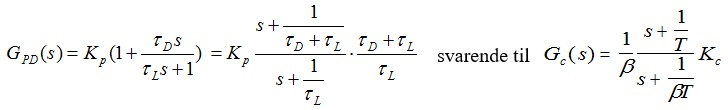
\includegraphics[width=1\linewidth]{graphics/lead_regulator}
	\label{fig:leadregulator}
\end{figure}
\\Se eksempel på Matlabkode i Appendix.

\newpage	
\section{Øvelsen}
Se systemoversigten ovenfor.\\

\noindent Direkte på motorakslen tilsluttes et 10-turns-potentiometer til vinkelmåling, skub potentiometeret frem til indgreb med udgangsakslen. Over potentiometeret lægges ±15V der hentes fra Control box via mini XLR-stik. Potentiometerets udtag er ført til BNC-stikket. Udtaget giver altså -15V for potentiometeret drejet helt til den ene side, og +15V for akslen drejet 10 omgange til den modsatte side.\\
\newline \textbf{Vigtigt!} \\
Teorien gælder kun så længe ingen af enhederne overstyres. Kontroller derfor udgangen på effekttrinnet ved alle målinger, udgangssignalet må ikke overstige ±20V
Benyt evt. 4-kanals scope, som vi dog kun har 10 af. Ved overstyring af Control box vil rød LED lyse, ±10V.

\begin{enumerate}
	\item Sæt på Control box Kp=1 og vippekontakten til x1. 
	Power Amplifier KPA=1.  Referencen, Vin = 0V (kan gøres ved blot at slukke funktionsgeneratoren).  Akslen skal nu dreje potentiometeret til sit midtpunkt.
	Prøv manuelt at dreje akslen, så vil du se, at positionen kan være både lidt over og under referencen. Grunden er at motoren først starter ved en spænding på 0,3-5V (friktion i lejer o.l. tør- og klæbe friktion ), det kan modelleres som en konstant forstyrrelse i blokdiagrammet.
	Slå Gain over på  x 10 og se at afvigelsen nu er meget mindre. Begrund forløbet.\\
	\item Brug funktionsgeneratoren indstillet til firkanter, ±200mV og 0,5 Hz, som reference.
	Juster forstærkningen KPA til et oversving < 5\%, ca. og sammenlign med forberedelsens Kc
	Iagttag positionens oversving og stationære fejl.
	(juster scopets offset så den stationære fejl er symmetrisk).\\
	\item Indstil funktionsgeneratoren til en trekantkurve, der går ±200 mV med frekvensen 0,5 Hz og iagttag den stationære fejl. Sammenlign med forberedelsen.\\
	\item Indsæt nu PI-regulatoren fra forberedelsen og iagttag den stationære fejl. Sammenlign med forberedelsen.\\
	\item Brug igen firkanter, ±200mV og 0,5 Hz som reference. Iagttag oversvinget.
	Formindsk Ti og iagttag variationen af \%OS. Forklar hvorfor.
	Formindsk i stedet forstærkningen og iagttag variationen af \%OS. Forklar hvorfor.\\
	\newline Efterfølgende anvendes PI-regulatoren ikke.\\
	\item Indstil forstærkningen KPA til 90, Brug firkanter, ±100mV og 0,5 Hz som reference og registrer oversvinget.\\
	\item Indstil forstærkningen KPA til 90, Brug firkanter, ±100mV og 0,5 Hz som reference og registrer oversvinget.\\
	\item Realiser den Lead-regulator du har dimensioneret under forberedelsen. Lav målinger og sammenlign med resultatet fra simuleringen. Juster evt. Kc, TD og TL til et bedre resultat.
	Kontroller effekttrinnet for evt. mætning.
\end{enumerate}

\newpage
\section{Bilag}
\subsection{Matlabkode}
\begin{lstlisting}[frame=single]
%% Forberedelse a)
clc
clear

s = tf('s');

N = 24;
Kc = 39;
Kpa = 1;
Gms = 720/(s+33);  
Kpot = 0.478;

G = Kc*Kpa*Gms*(1/s)*(1/N)*Kpot;

% Ved simulering findes den største værdi,
% for hvilken lukketsløjfe systemet har et oversving < 5%.
% Iagttag settlingtime, oversving og stationære fejl. 
figure(1)
F = feedback(G,1)
step(F)

% Plot for KC-værdien amplitude- og fasekarakteristik,
% og find den tilhørende fasemargin og fasemarginsfrekvens.
figure(2)
margin(G)
\end{lstlisting}

\end{document}          
